\documentclass[9pt,aspectratio=169,xcolor=table]{beamer}

%~~~~~~~~~~~~~~~~~~~~~~~~~~~~~~~~~~~~~~~~~~~~~~~~~~~~~~~~~~~~~~~~~~~~~~~~~~~~~~
% Use roboto Font (recommended)
\usepackage[sfdefault]{roboto}
\usepackage[utf8]{inputenc}
\usepackage[T1]{fontenc}
%~~~~~~~~~~~~~~~~~~~~~~~~~~~~~~~~~~~~~~~~~~~~~~~~~~~~~~~~~~~~~~~~~~~~~~~~~~~~~~

%~~~~~~~~~~~~~~~~~~~~~~~~~~~~~~~~~~~~~~~~~~~~~~~~~~~~~~~~~~~~~~~~~~~~~~~~~~~~~~
% Define where theme files are located. ('/styles')
\usepackage{styles/fluxmacros}
\usefolder{styles}
% Use Flux theme v0.1 beta
% Available style: asphalt, blue, red, green, gray
\usetheme[style=hunter]{flux}
%~~~~~~~~~~~~~~~~~~~~~~~~~~~~~~~~~~~~~~~~~~~~~~~~~~~~~~~~~~~~~~~~~~~~~~~~~~~~~~

%~~~~~~~~~~~~~~~~~~~~~~~~~~~~~~~~~~~~~~~~~~~~~~~~~~~~~~~~~~~~~~~~~~~~~~~~~~~~~~
% Extra packages
\usepackage{booktabs}
\usepackage{colortbl}
\usepackage{ragged2e}
\usepackage{amssymb}
\usepackage{multirow}
\usepackage{tikz}
\usetikzlibrary{arrows.meta, positioning, fit, backgrounds, calc, decorations.pathreplacing}
\setbeamertemplate{itemize items}[square]
\usepackage[scaled=.8]{beramono}
\usepackage{listings}
\usepackage{styles/lstlangarm}
\usepackage{array}
\definecolor{bgcolor}{HTML}{F2E9E9}
% lstlangarm.sty references \color{mauve} for string literals but never defines
% it -- only fires when a listing contains a string. Define it here.
\definecolor{mauve}{rgb}{0.58,0,0.82}
% lstlangarm's C style sets commentstyle=green!20, which is unreadable on the
% pink listing background. Darken it globally.
\lstset{commentstyle=\color{green!45!black}}
% ragged-right fixed-width column -- must be defined in the preamble, never
% inside a frame (\newcolumntype's #1 breaks beamer's frame scanner)
\newcolumntype{R}[1]{>{\RaggedRight\arraybackslash}p{#1}}
%~~~~~~~~~~~~~~~~~~~~~~~~~~~~~~~~~~~~~~~~~~~~~~~~~~~~~~~~~~~~~~~~~~~~~~~~~~~~~~
% Table striping: odd rows white, even rows very light gray.
% Needs \documentclass[...,xcolor=table]{beamer} (beamer loads xcolor itself,
% so the option must go on the class, not \usepackage).
\definecolor{stripe}{gray}{0.94}
% \striped makes body rows alternate white, gray, white, ... starting white.
% \rowcolors counts from the first coloured body row; the header is not counted.
\newcommand{\striped}{\rowcolors{1}{white}{stripe}}
%~~~~~~~~~~~~~~~~~~~~~~~~~~~~~~~~~~~~~~~~~~~~~~~~~~~~~~~~~~~~~~~~~~~~~~~~~~~~~~

%~~~~~~~~~~~~~~~~~~~~~~~~~~~~~~~~~~~~~~~~~~~~~~~~~~~~~~~~~~~~~~~~~~~~~~~~~~~~~~
% TikZ block styles -- matches ch1/ch2
% Colour variables are named identically in the book's stm32primer.tex, so any
% tikzpicture using only the \tikzset{...} styles below can be copied verbatim
% between slides and book. Only the \definecolor/\colorlet VALUES differ: the
% book is printed, so it keeps every stroke pure black with muted fills. These
% slides are projected, so both fill AND stroke are bright and saturated to
% grab attention -- see stm32primer.tex for the print palette.
\definecolor{blkfill}{HTML}{DDEEDD}
\definecolor{blkline}{HTML}{355E3B}
\definecolor{accentfill}{HTML}{FFE0B2}
\definecolor{accentline}{HTML}{E65100}
\definecolor{memfill}{HTML}{DFF5DA}
\definecolor{memline}{HTML}{2E7D32}
\definecolor{cellfill}{HTML}{FFFFFF}
\definecolor{cellline}{HTML}{424242}
\definecolor{bitmaskfill}{HTML}{DCEBFF}
\definecolor{bitmaskline}{HTML}{1565C0}
\definecolor{bithitfill}{HTML}{FFE0B2}
\definecolor{bithitline}{HTML}{E65100}
\tikzset{
  blk/.style   = {rectangle, rounded corners=2pt, draw=blkline, fill=blkfill,
                  thick, align=center, font=\small, minimum height=9mm, inner sep=3pt},
  cpublk/.style= {rectangle, rounded corners=2pt, draw=accentline, fill=accentfill,
                  thick, align=center, font=\small\bfseries, minimum height=9mm, inner sep=3pt},
  memblk/.style= {rectangle, rounded corners=2pt, draw=memline, fill=memfill,
                  thick, align=center, font=\small, minimum height=9mm, inner sep=3pt},
  cell/.style  = {rectangle, draw=cellline, fill=cellfill, align=center,
                  font=\small\ttfamily, minimum height=7mm, inner sep=2pt},
  bitcell/.style={rectangle, draw=cellline, fill=cellfill, thick,
                  minimum width=5.4mm, minimum height=5.4mm, inner sep=0pt,
                  font=\scriptsize\ttfamily, anchor=center},
  bitmask/.style={bitcell, fill=bitmaskfill, draw=bitmaskline},
  bithit/.style ={bitcell, fill=bithitfill, draw=bithitline, font=\scriptsize\ttfamily\bfseries},
  rowlab/.style ={font=\scriptsize, text=Gray, anchor=east},
  oplab/.style  ={font=\scriptsize\itshape, text=Gray, anchor=west},
  lbl/.style   = {font=\scriptsize, text=Gray},
  flow/.style  = {-{Stealth[length=2mm]}, thick, draw=blkline},
  busline/.style={thick, draw=cellline},
}
% NOTE (theme quirks -- all fail SILENTLY, always page through the PDF):
%  - a second \\ inside a nested {...} group in a TikZ node breaks parsing
%  - {\small ...} wrapped around a nested itemize eats the frame title + list
%  - \usebeamercolor on a [plain] frame falls through to an unstyled default
%  - \newcolumntype inside a frame breaks beamer's frame scanner
%  - lstlisting needs \begin{frame}[fragile]
%  - a TikZ picture wider than its column silently overflows into neighbours
%~~~~~~~~~~~~~~~~~~~~~~~~~~~~~~~~~~~~~~~~~~~~~~~~~~~~~~~~~~~~~~~~~~~~~~~~~~~~~~

%%%%%%%%%%%%%%%%%%%%%%%%%%%%%%%%%%%
%% BEGIN CONDITIONAL COMPILATION %%
%%%%%%%%%%%%%%%%%%%%%%%%%%%%%%%%%%%
\newif\ifwebex
%\webextrue % uncomment to generate section separator
\ifwebex
\AtBeginSection[]{
  \begin{frame}
  \vfill
  \centering
  \begin{beamercolorbox}[sep=8pt,center,shadow=true,rounded=true]{title}
    \usebeamerfont{title}\insertsectionhead\par%
  \end{beamercolorbox}
  \vfill
  \end{frame}
}
\else
\AtBeginSection[]
{
{
    \setbeamercolor{background canvas}{bg=yellow!10}
    \begin{frame}[plain]
        \frametitle{Table of Contents}
        \tableofcontents[currentsection]
    \end{frame}
}
}
\fi
%%%%%%%%%%%%%%%%%%%%%%%%%%%%%%%%%%%
%% END CONDITIONAL COMPILATION   %%
%%%%%%%%%%%%%%%%%%%%%%%%%%%%%%%%%%%

%~~~~~~~~~~~~~~~~~~~~~~~~~~~~~~~~~~~~~~~~~~~~~~~~~~~~~~~~~~~~~~~~~~~~~~~~~~~~~~
% Information
\title{Counters}
\subtitle{\emph{Contemporary Digital Electronic Systems} --- Chapter 12}
\author{Mun\'{i}m Zabidi}
\institute{\color{primary}Faculty of Electrical Engineering, Universiti Teknologi Malaysia}
\date{\today}
\titlegraphic{assets/logoutmwhite.png}
\graphicspath{{.}{../fig/}}
%~~~~~~~~~~~~~~~~~~~~~~~~~~~~~~~~~~~~~~~~~~~~~~~~~~~~~~~~~~~~~~~~~~~~~~~~~~~~~~

\newcommand{\figh}[2]{\includegraphics[height=#1\textheight]{#2}}



\begin{document}

\titlepage

%===============================================================================
\section{Why This Chapter}
%===============================================================================

\begin{frame}{Why This Chapter Matters}
  \begin{columns}[c]
  \begin{column}{.47\textwidth}
    Counters are the simplest and most widely used sequential circuits: every digital clock, timer, frequency divider and sequence generator contains one. They are also the first circuits where the \alert{state is read as a number}, a bridge from registers to the state-based thinking of Chapters 13--15.
  \end{column}
  \begin{column}{.51\textwidth}
    \begin{block}{After this chapter, you can:}
    {\small
    \begin{enumerate}\itemsep2pt
      \item Design asynchronous (ripple) counters of any modulus and explain their limitation.
      \item Design synchronous binary up counters.
      \item Design a modulo-$N$ counter ($N$ not a power of two), such as a decade counter, with the synchronous design procedure.
      \item Use a counter as a frequency divider.
    \end{enumerate}}
    \end{block}
  \end{column}
  \end{columns}
\end{frame}

\begin{frame}{An Opening Question}
  \leavevmode\vspace{4mm}
  \begin{center}
  \fbox{\parbox{.78\textwidth}{\centering\vspace{2mm}
  \large A 50\,MHz clock drives an LED that should blink once per second. What is the \alert{modulus} of the counter between them?
  \vspace{2mm}}}
  \end{center}
  \vspace{4mm}
  We answer this with the frequency-division property of counters.
\end{frame}

%===============================================================================
\section{Introduction}
%===============================================================================

\begin{frame}{What Is a Counter?}
  \begin{itemize}\small\itemsep3pt
    \item A series of flip-flops whose outputs form a binary number; each clock pulse increments the count.
    \item Key difference, the clocking method:
    \begin{itemize}\small
      \item \alert{Asynchronous (ripple)}: each stage's output clocks the next; stages change one after another.
      \item \alert{Synchronous}: one common clock; all outputs change together.
    \end{itemize}
    \item Other classifications: modulus, count direction (up, down, up/down), edge polarity, flip-flop type.
    \item \alert{Modulus} (mod) = number of states. $n$ flip-flops give up to $2^n$ states: a 3-bit counter is mod-8.
    \item A counter with fewer than $2^n$ states is \alert{truncated}: a decade (mod-10) counter counts 0000 to 1001.
  \end{itemize}
\end{frame}

%===============================================================================
\section{Asynchronous Counters}
%===============================================================================

\begin{frame}{2-Bit Ripple Counter}
  \begin{columns}[c]
  \begin{column}{.5\textwidth}
    \centering
    \figh{.2}{ctr_ripple2bit_jkff}\\[2mm]
    \centering\small\striped
    \begin{tabular}{@{}ccc@{}}
      \toprule
      Clock & $Q_B$ & $Q_A$ \\
      \midrule
      Initial & 0 & 0 \\ 1 & 0 & 1 \\ 2 & 1 & 0 \\ 3 & 1 & 1 \\ 4 & 0 & 0 \\
      \bottomrule
    \end{tabular}
  \end{column}
  \begin{column}{.48\textwidth}
    \begin{itemize}\small\itemsep3pt
      \item The external clock drives only flip-flop A. Each falling edge toggles A.
      \item When A falls from 1 to 0, B toggles.
    \end{itemize}
    \centering
    \figh{.2}{ctr_ripple2bit_td}\hspace{2mm}\figh{.2}{ctr2bit_sd}
  \end{column}
  \end{columns}
\end{frame}

\begin{frame}{3-Bit Ripple Counter}
  \centering
  \figh{.2}{ctr_ripple3bit_jkff}\hspace{4mm}\figh{.2}{ctr3bit_sd}\\[2mm]
  \figh{.25}{ctr_ripple3bit_td}
  \begin{itemize}\small\itemsep2pt
    \item $2^3 = 8$ states: mod-8.
    \item Any flip-flop that can toggle works: T, JK with $J = K = 1$, or D with $\overline{Q}$ fed back to $D$.
  \end{itemize}
\end{frame}

\begin{frame}{Ripple Counters Divide Frequency}
  \begin{itemize}\small\itemsep3pt
    \item Each flip-flop divides its clock by 2. With an 8 kHz clock, A, B and C output 4 kHz, 2 kHz and 1 kHz.
    \item A counter of modulus $N$ divides the input frequency by $N$ (if it cycles through its $N$ states once per period).
  \end{itemize}
  \begin{block}{An answer to the opening question}
    \small 50 MHz to 1 Hz needs division by $50\,000\,000$: a counter of modulus $50\,000\,000$ ($\lceil\log_2 50\,000\,000\rceil = 26$ flip-flops). A divide-by-$N$ counter turns an $f$ Hz clock into $f/N$ Hz.
  \end{block}
\end{frame}

\begin{frame}{Limitation: Cumulative Propagation Delay}
  \begin{columns}[c]
  \begin{column}{.5\textwidth}
    \centering
    \figh{.3}{exaggerated_delays}
  \end{column}
  \begin{column}{.48\textwidth}
    \begin{itemize}\small\itemsep3pt
      \item Each stage waits for the previous one, so changes \alert{ripple}.
      \item With delay $t_p$ per stage, the output settles about $nt_p$ after the clock edge:
    \end{itemize}
    \[ T \ge nt_p, \qquad f_{\max} \le \frac{1}{nt_p} \]
    \small Simplified model: it ignores other timing requirements.
  \end{column}
  \end{columns}
  \begin{block}{Example: 4-bit counter, $t_p = 12$ ns}
    \small $nt_p = 48$ ns, so $f_{\max} \le 20.8$ MHz. Modulus 16: output at the last stage is about $20.8/16 \approx 1.3$ MHz.
  \end{block}
\end{frame}

\begin{frame}{False (Ghost) States}
  \begin{columns}[c]
  \begin{column}{.55\textwidth}
    \centering
    \figh{.25}{false_counts}\hspace{2mm}\figh{.25}{false_states}
  \end{column}
  \begin{column}{.43\textwidth}
    \begin{itemize}\small\itemsep3pt
      \item Transition $011 \to 100$: A toggles ($010$), B toggles ($000$), C toggles ($100$).
      \item The intermediate states are temporary results of delay, not part of the sequence.
      \item They matter if other circuits read the outputs as a number while they are changing. Sample only after settling.
    \end{itemize}
  \end{column}
  \end{columns}
  \vspace{2mm}
  {\small If a ripple counter is used only for frequency division, unused stages may be less restrictive; still check the flip-flop specifications.}
\end{frame}

%===============================================================================
\section{Synchronous Counters}
%===============================================================================

\begin{frame}{Synchronous Binary Counters}
  \begin{columns}[c]
  \begin{column}{.62\textwidth}
    \centering
    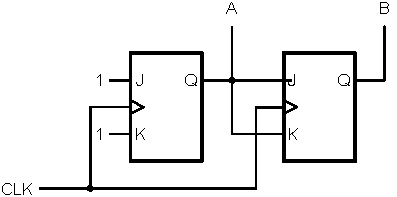
\includegraphics[scale=.58]{ctr_sync2bit_jkff}\\[-1mm]{\scriptsize 2-bit, mod-4}\\[2mm]
    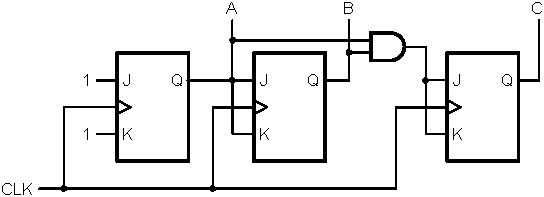
\includegraphics[scale=.58]{ctr_mod8}\\[-1mm]{\scriptsize 3-bit, mod-8}\\[2mm]
    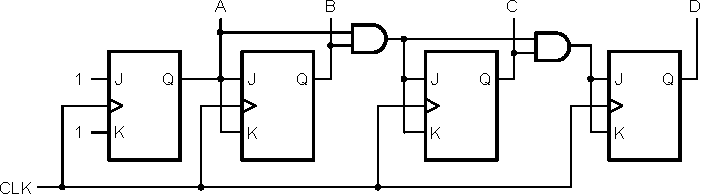
\includegraphics[scale=.58]{ctr_mod16}\\[-1mm]{\scriptsize 4-bit, mod-16}
  \end{column}
  \begin{column}{.36\textwidth}
    \begin{itemize}\small\itemsep4pt
      \item One clock for every flip-flop: outputs change together, with no stage-to-stage delay.
      \item The LSB toggles on every pulse; each higher bit toggles only when \alert{all lower bits are 1}. Combinational logic (AND gates) detects this.
      \item Costs extra logic, but runs faster.
    \end{itemize}
  \end{column}
  \end{columns}
\end{frame}

\begin{frame}{Decade Counter and Speed}
  \begin{columns}[c]
  \begin{column}{.5\textwidth}
    \centering
    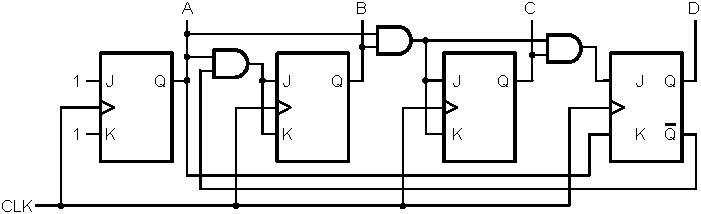
\includegraphics[width=.95\textwidth]{ctr_mod10}\\[1mm]
    {\small Mod-10: counts 0000 to 1001, then 0000}
  \end{column}
  \begin{column}{.48\textwidth}
    \begin{itemize}\small\itemsep3pt
      \item Four flip-flops could hold 16 states, but this counter uses only ten.
      \item The longest path is one AND gate plus one flip-flop: $f_{\max} \le 1/(t_g + t_f)$: the delay does not accumulate stage by stage. The MSB AND gate widens with $n$ and becomes a gate tree, so the delay grows only with $\log n$.
    \end{itemize}
    \begin{block}{Example: $t_f = 12$ ns, $t_g = 5$ ns}
      \small $f_{\max} \le 1/17\ \text{ns} \approx 58.8$ MHz, about $2.8\times$ the ripple counter's 20.8 MHz.
    \end{block}
  \end{column}
  \end{columns}
\end{frame}

%===============================================================================
\section{Design of Synchronous Counters}
%===============================================================================

\begin{frame}{Counter Design Procedure}
  \begin{columns}[c]
  \begin{column}{.45\textwidth}
    \centering
    \figh{.25}{counterarchitecture}
  \end{column}
  \begin{column}{.53\textwidth}
    \centering
    \figh{.35}{counter_synthesis}
  \end{column}
  \end{columns}
  \begin{itemize}\small\itemsep3pt
    \item A synchronous counter is flip-flops plus next-state logic: the counting sequence is set by that logic. This is finite-state-machine design (next chapter).
    \item Non-D flip-flops need an \alert{excitation table}. For D flip-flops the input simply equals the desired next state.
  \end{itemize}
\end{frame}

\begin{frame}{Design with D Flip-Flops: 2-Bit Counter}
  \begin{columns}[c]
  \begin{column}{.45\textwidth}
    \centering
    \figh{.2}{mod4ctr_sd}\\[2mm]
    \small\striped
    \begin{tabular}{@{}cc|cc|cc@{}}
      \toprule
      $Q_1$ & $Q_0$ & $Q_1^+$ & $Q_0^+$ & $D_1$ & $D_0$ \\
      \midrule
      0&0&0&1&0&1 \\ 0&1&1&0&1&0 \\ 1&0&1&1&1&1 \\ 1&1&0&0&0&0 \\
      \bottomrule
    \end{tabular}
  \end{column}
  \begin{column}{.53\textwidth}
    \begin{enumerate}\small\itemsep2pt
      \item State diagram: arrows are unconditional.
      \item State table: next state for each present state.
      \item Flip-flop inputs: $D = Q^+$.
      \item Equations by inspection:
    \end{enumerate}
    \[ D_1 = Q_1 \oplus Q_0 \qquad D_0 = \overline{Q_0} \]
    \begin{enumerate}\small\setcounter{enumi}{4}
      \item Implement.
    \end{enumerate}
    \centering
    \figh{.2}{mod4ctr_cs}
  \end{column}
  \end{columns}
\end{frame}

\begin{frame}{Example: Mod-5 Counter with D Flip-Flops}
  \begin{columns}[c]
  \begin{column}{.5\textwidth}
    \centering\scriptsize\striped
    \begin{tabular}{@{}ccc|ccc@{}}
      \toprule
      $Q_2$ & $Q_1$ & $Q_0$ & $Q_2^+$ & $Q_1^+$ & $Q_0^+$ \\
      \midrule
      0&0&0&0&0&1 \\ 0&0&1&0&1&0 \\ 0&1&0&0&1&1 \\ 0&1&1&1&0&0 \\ 1&0&0&0&0&0 \\
      1&0&1&x&x&x \\ 1&1&0&x&x&x \\ 1&1&1&x&x&x \\
      \bottomrule
    \end{tabular}
  \end{column}
  \begin{column}{.48\textwidth}
    \begin{itemize}\small\itemsep3pt
      \item Three unused states (101, 110, 111): their next states are don't cares.
      \item K-maps with the don't cares give:
    \end{itemize}
    \small
    $D_2 = Q_1Q_0$\\
    $D_1 = \overline{Q_2}\,\overline{Q_0}Q_1 + \overline{Q_2}\,\overline{Q_1}Q_0$\\
    $D_0 = \overline{Q_2}\,\overline{Q_0}$
    \begin{block}{Check self-correction}
      \small State 101 gives $D_2D_1D_0 = 000$: it returns to 000 next clock. Always verify this: don't-care simplification does not guarantee it.
    \end{block}
  \end{column}
  \end{columns}
\end{frame}

\begin{frame}{Design with T Flip-Flops: Mod-8 Counter}
  \begin{columns}[c]
  \begin{column}{.55\textwidth}
    \centering\tiny\striped
    \begin{tabular}{@{}ccc|ccc|ccc@{}}
      \toprule
      $Q_2$ & $Q_1$ & $Q_0$ & $Q_2^+$ & $Q_1^+$ & $Q_0^+$ & $T_2$ & $T_1$ & $T_0$ \\
      \midrule
      0&0&0&0&0&1&0&0&1 \\ 0&0&1&0&1&0&0&1&1 \\ 0&1&0&0&1&1&0&0&1 \\ 0&1&1&1&0&0&1&1&1 \\
      1&0&0&1&0&1&0&0&1 \\ 1&0&1&1&1&0&0&1&1 \\ 1&1&0&1&1&1&0&0&1 \\ 1&1&1&0&0&0&1&1&1 \\
      \bottomrule
    \end{tabular}\\[2mm]
    \figh{.2}{ctr_mod8_sd}
  \end{column}
  \begin{column}{.43\textwidth}
    \begin{itemize}\small\itemsep3pt
      \item A T input is 1 when the flip-flop must change.
      \item K-maps give $T_2 = Q_1Q_0$, $T_1 = Q_0$, $T_0 = 1$.
    \end{itemize}
    \centering
    \figh{.12}{ctr_mod8_kmap1}\hspace{1mm}\figh{.12}{ctr_mod8_kmap2}\hspace{1mm}\figh{.12}{ctr_mod8_kmap3}
  \end{column}
  \end{columns}
\end{frame}

\begin{frame}{Mod-8 Counter Schematic and the General Rule}
  \begin{columns}[c]
  \begin{column}{.5\textwidth}
    \centering
    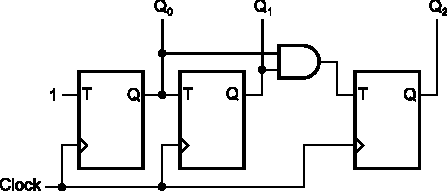
\includegraphics[width=.95\textwidth]{ctr_mod8_sc_tff}
  \end{column}
  \begin{column}{.48\textwidth}
    \begin{block}{General rule for $n$-bit T-flip-flop up counters}
      \[ T_i = Q_{i-1}Q_{i-2}\cdots Q_1Q_0,\quad T_0 = 1 \]
      \small Bit $i$ toggles exactly when all lower bits are 1 (the ripple-carry condition).
    \end{block}
    \small A 4-bit counter needs $T_3 = Q_2Q_1Q_0$ with no fourth K-map. T flip-flops suit binary up counters: each $T_i$ is a simple AND, unlike the D-flip-flop expressions.
  \end{column}
  \end{columns}
\end{frame}

\begin{frame}{Back to the Opening Question}
  \begin{block}{Blinking an LED once per second}
    \small The counter divides $50\,000\,000$ Hz down to 1 Hz, so its modulus is $50\,000\,000$. That needs 26 flip-flops and is not a power of two, so the counter must be truncated (design it with the modulo-$N$ procedure). A ripple version would be far too slow at 50 MHz, so a synchronous design is the sensible choice.
  \end{block}
\end{frame}

%===============================================================================
\section{Summary}
%===============================================================================

\begin{frame}{Summary}
  \begin{itemize}\itemsep3pt\small
    \item An \alert{asynchronous (ripple) counter} clocks each stage from the previous one: simple, but delay accumulates and limits speed.
    \item A \alert{synchronous counter} clocks every flip-flop together: faster, with more logic.
    \item Modulo-$N$ counters ($N$ not a power of two), such as a decade counter, are designed with the synchronous design procedure; check unused states for self-correction.
    \item A counter divides frequency by its modulus: divide-by-$N$ turns $f$ Hz into $f/N$ Hz.
  \end{itemize}
  \begin{block}{Looking ahead}
    Counters give an \emph{ordered} sequence of states. When the next state depends on inputs, we need a \emph{finite state machine}: Chapters 13--15.
  \end{block}
\end{frame}

\end{document}
